\subsubsection*{Phần A: Cân bằng}
\begin{figure}[H]
  \centering
  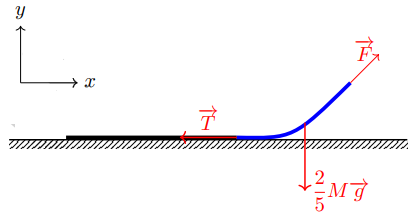
\includegraphics[width=0.45\textwidth]{Figures/Solutions/Fig 3.1.png}
\end{figure}
\vspace{-0.5cm}

\noindent Cân bằng lực đối với đoạn dây không chạm đất:
\begin{equation*}
  \frac{2}{5} M \vec{g} + \vec{T} + \vec{F} = \vec{0}
\end{equation*}
Chiếu lên các trục toạ độ, ta có:
\begin{equation*}
  \frac{2}{5}Mg = F_y
\end{equation*}
\begin{equation*}
  T = F_x
\end{equation*}
\begin{figure}[H]
  \centering
  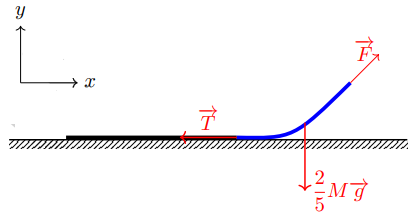
\includegraphics[width=0.5\textwidth]{Figures/Solutions/Fig 3.1.png}
\end{figure}
\vspace{-0.5cm}

\noindent Điều kiện cân bằng của đoạn dây nằm trên bàn:
\begin{equation*}
  T \leq \frac{3}{5} \mu M g
\end{equation*}
Lưu ý rằng, lực căng dây tại hai phần của sợi dây là có độ lớn bằng nhau, ta có:
\begin{equation*}
  F^2 = F_x^2 + F_y^2 \leq \left( \frac{2}{5}Mg \right)^2 + \left( \frac{3}{5} \mu Mg \right)^2 = \left( \frac{1}{5}Mg \right)^2 \left[ 4 + (3\mu)^2 \right]
\end{equation*}
Suy ra:
\begin{equation*}
  \mu \geq \frac{1}{3} \sqrt{ \left( \frac{5F}{Mg} \right)^2 - 4 }
\end{equation*}

\subsubsection*{Phần B: Quay đầu}
\noindent Định luật II Newton:
\begin{equation*}
  F = \frac{dp}{dt}
\end{equation*}
Trong đó $F$ là lực do Alice tác dụng và $p$ là động lượng của phần dây di chuyển. Gọi $m$ và $l$ là khối lượng và chiều dài của phần dây di chuyển, ta có:
\begin{equation*}
  \frac{dp}{dt} = v \frac{dm}{dt} = \frac{vM}{L} \frac{dl}{dt}
\end{equation*}
Xét một đoạn dây có chiều dài $dl$, khi toàn bộ đoạn dây này di chuyển, Alice phải đi một đoạn dài gấp đôi chiều dài đoạn dây, do đó:
\begin{equation*}
  \frac{dl}{dt} = \frac{v}{2}
\end{equation*}
Suy ra:
\begin{equation*}
  F = \frac{Mv^2}{2L}
\end{equation*}

\subsubsection*{Phần C: Trượt khỏi bàn}
\noindent\textbf{1.} Gọi $x$ là chiều dài đoạn dây buông ngoài mép bàn.
\begin{figure}[H]
  \centering
  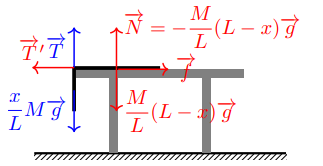
\includegraphics[width=0.4\textwidth]{Figures/Solutions/Fig 3.3.png}
\end{figure}
\vspace{-0.5cm}

\noindent Năng lượng ban đầu:
\begin{equation*}
  E_i = -\frac{l_0^2Mg}{2L}
\end{equation*}
Năng lượng lúc sau:
\begin{equation*}
  E_f = -\frac{MgL}{2} + \frac{Mv_f^2}{2}
\end{equation*}
Công thực hiện bởi lực ma sát:
\begin{equation*}
  W = \int_{l_0}^{L} \frac{M}{L}(L - x)\mu g dx = \frac{(L - l_0)^2 \mu Mg}{2L}
\end{equation*}
Định luật bảo toàn năng lượng:
\begin{equation*}
  E_i + W = E_f
\end{equation*}
Suy ra:
\begin{equation*}
  v_f=\sqrt{\frac{(L-l_0)^2 g}{L}\mu-\frac{l_0^2 g}{L}+gL}
\end{equation*}

\noindent\textbf{2.} Vì dây không dãn, gia tốc tại mọi điểm trên sợi dây là như nhau. Theo định luật II Newton:
\begin{equation*}
  F = \frac{dp}{dt} = M \ddot{x}
\end{equation*}
\begin{equation*}
  M \ddot{x} = \frac{M}{L} x g - \frac{M}{L} (L - x) \mu g
\end{equation*}
Suy ra:
\begin{equation*}
  \ddot{x} = \frac{g}{L} (\mu + 1) x - \mu g
\end{equation*}

\noindent\textbf{3.} Ta có thể viết $x(t)$ dưới dạng:
\begin{equation*}
  x(t) = A \cosh(\omega t) + B
\end{equation*}
Lưu ý rằng $\cosh'' t = \cosh t$, ta có:
\begin{equation*}
  A \omega^2 \cosh(\omega t) = (A \cosh(\omega t) + B) \frac{g}{L} (\mu + 1) - \mu g
\end{equation*}
Từ đó ta tìm được:
\begin{equation*}
  \omega^2 = \frac{g}{L} (\mu + 1)
\end{equation*}
Và:
\begin{equation*}
  B = \frac{\mu}{\mu + 1} L
\end{equation*}
Cuối cùng, hệ số $A$ được xác định thông qua điều kiện ban đầu $x(0) = l_0$:
\begin{equation*}
  x(0) = A \cosh(0) + B = A + B = l_0 \Rightarrow A = l_0 - B = l_0 - \frac{\mu}{\mu + 1} L
\end{equation*}

\subsubsection*{Phần D: Treo vật}
\noindent Vì sợi dây không dãn, lực căng dây tại mọi điểm trên sợi dây là như nhau. Bỏ qua số hạng $\dot{r}$, các phương trình chuyển động là:
\begin{equation*}
  \left\{
  \begin{aligned}
     & - m \ddot{r}                    = - m g - T             \\
     & m r \ddot{\theta}               = - m g \sin \theta     \\
     & m(\ddot{r} - r \dot{\theta}^2)  = - m g \cos \theta + T
  \end{aligned}
  \right.
\end{equation*}
Loại bỏ $T$, ta được:
\begin{equation*}
  \left\{
  \begin{aligned}
     & \ddot{r}                      = - g \sin \theta     \\
     & 2 \dot{r} - r \dot{\theta}^2  = g (\cos \theta - 1)
  \end{aligned}
  \right.
\end{equation*}
Đối với góc nhỏ
\begin{equation*}
  \left\{
  \begin{aligned}
     & r \ddot{\theta}               = - g \theta               \\
     & 2 \dot{r} - r \dot{\theta}^2  = - \frac{1}{2} g \theta^2
  \end{aligned}
  \right.
\end{equation*}
Sử dụng điều kiện ban đầu và nghiệm
\begin{equation*}
  \theta(t) = \varepsilon \omega \sin(\omega t)
\end{equation*}
Với $\omega^2 = \frac{g}{r}$. Lưu ý rằng, ở đây $r$ có thể xem như là hằng số (trong một chu kì dao động), do đó $\dot{r} \approx 0$. Từ phương trình thứ hai suy ra:
\begin{align*}
  2 \ddot{r} & = - \frac{1}{2} g \theta^2 + r \dot{\theta}^2                                              \\
             & = - \frac{1}{2} g \varepsilon^2 \cos^2(\omega t) + r\varepsilon^2\omega^2 \sin^2(\omega t) \\
             & = - \frac{1}{2} g \varepsilon^2 \cos^2(\omega t) + g \varepsilon^2 \sin^2(\omega t)
\end{align*}
Gia tốc trung bình trong một chu kì dao động
\begin{equation*}
  \langle \ddot{r} \rangle = \frac{1}{2} g \varepsilon^2 \left( \frac{1}{2} \int_0^{2\pi/\omega} \cos^2(\omega t) \, dt + \int_0^{2\pi/\omega} \sin^2(\omega t) \, dt \right)
  = \frac{3 \pi}{4}  \frac{g \varepsilon^2}{\omega}
\end{equation*}